\documentclass[journal,onecolumn]{IEEEtran}
\usepackage[T1]{fontenc}
\ifCLASSINFOpdf
\else
\fi
\hyphenation{op-tical net-works semi-conduc-tor}
\usepackage{enumitem}
\usepackage{caption}
\captionsetup{justification   = raggedright,
              singlelinecheck = false}
\usepackage{graphicx}
\usepackage{subfigure}
\usepackage{svg}
\usepackage{siunitx}
\usepackage{xcolor}
\usepackage{hyperref}
\begin{document}

\title{Replikácia článku\\ A New Deep Learning Model for the Classification of
Poisonous and Edible Mushrooms Based on Improved AlexNet
Convolutional Neural Network}

\author{Ján~Schmiedbauer,
        Valér~Tóth}


\markboth{Marec~2025}%
{Shell \MakeLowercase{\textit{et al.}}: Bare Demo of IEEEtran.cls for IEEE Journals}

\maketitle
\IEEEpeerreviewmaketitle

\section{Sumarizácia článku a problematiky}

\IEEEPARstart{N}{áš} článok \cite{pc} je od autorov Wacharaphol Ketwongsa \cite{wk}, Sophon Boonlue a Urachart Kokaew \cite{uk}, ktorí sú všetci členovia univerzity Khon Kaen \cite{kk}, ktorá sa nachádza v Thajsku. Hlavná problematika článku sa týka rozpoznávania jedlých a jedovatých húb pomocou CNN a tiež aj RCNN. Článok bol čiastočne motivovaný každoročnými smrťami, ktoré sa uskutočňujú ako dôsledok konzumácie jedovatých húb v Thajsku a autori dúfajú, že výskum klasifikačných technológií môže pomôcť predísť takýmto incidentom. Tiež sú spomenuté rôzne tradičné spôsoby rozpoznávania jedovatých húb v Thajsku a ich relatívna neefektivnosť.V článku "Toxíny v sebe nemajú iba muchotrávky: Lekárka radí, čo robiť, ak sa otrávite hubami" \cite{nc} od publikácie Nový čas je zverejnená štatistika, že približne 100 až 120 Slovákov je ročne hospitalizovaných kvôli otrave jedovatými hubami, čiže táto problematika je relevantná aj pre nás na Slovensku.

\IEEEPARstart{}{}
Hlavnou témou článku je návrh nového CNN modelu založeného na báze známeho modelu AlexNet. Tento nový model bol porovnaný s tromi predtrénovanými architektúrami : GoogleNet (InceptionV1), ResNet50, a tiež aj so samotným AlexNet. Súčasťou porovnania bola tiež efektívnosť CNN ako súčasť RCNN. Všetky modely boli pomocou transfer learning metód pretrénované a testované na datasete 2000 obrázkov rôznych húb a bolo zistené, že navrhnutý model síce nepresahoval presnosť porovnávaných modelov, ale vedel získať podobné (vysoké) hodnoty za menší čas. Pre CNN 98.50\% a pre RCNN 95.50\%.

\section{Dataset}

\IEEEPARstart{P}{ôvodný} dataset obsahoval 623 obrázkov 5 rôznych druhov jedlých a jedovatých húb s veľkosťou 227 X 227 X 3 pixelov. Súčasťou jedlých druhov boli :
\begin{enumerate}[label=\Alph*]
  \item {\it Amanita citrina} (Muchotrávka citronožltá)
  \item {\it Russula delica} (Plávka belavá)
  \item {\it Phaeogyroporus portentosus} (Phlebopus marginatus)
\end{enumerate}

\IEEEPARstart{}{}
A jedovatých druhov :
\begin{enumerate}[label=\Alph*]
  \setcounter{enumi}{3}
  \item {\it Inocybe rimosa} (Vláknica kuželovitá)
  \item {\it Amanita phalloides} (Muchotrávka zelená)
\end{enumerate}

%\IEEEPARstart{}{} Táto tabuľka popisuje početnosť všetkých druhov v pôvodnom 
% datasete :

\captionof{table}{Početnosť v pôvodnom datasete}
\begin{center}
{\renewcommand{\arraystretch}{1.5}
\begin{tabular}{ccccc}
\hline
\multicolumn{3}{c}{Jedlé} 
&                                            
\multicolumn{2}{c}{Jedovaté} \\
\hline          
Muchotrávka citronožltá & Plávka belavá & Phlebopus marginatus & Vláknica kuželovitá & Muchotrávka zelená \\
248 & 88 & 155 & 76 & 56
\end{tabular}}
\end{center}

\begin{figure}[!htb]
    \centering
    \subfigure[]{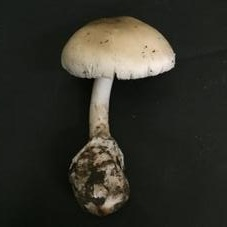
\includegraphics[width=0.14\textwidth]{Images/MCZ.jpg}} 
    \subfigure[]{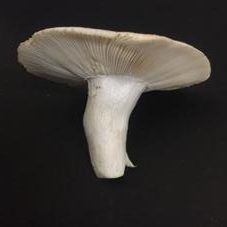
\includegraphics[width=0.14\textwidth]{Images/PB.jpg}} 
    \subfigure[]{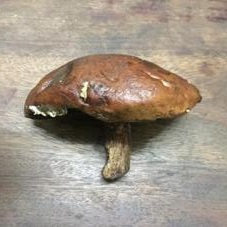
\includegraphics[width=0.14\textwidth]{Images/PM.jpg}}
    \subfigure[]{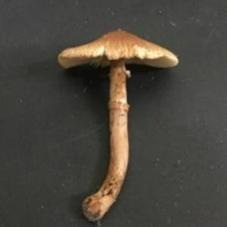
\includegraphics[width=0.14\textwidth]{Images/VK.jpg}}
    \subfigure[]{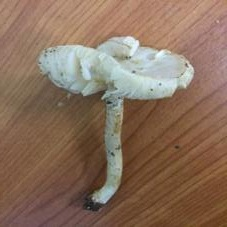
\includegraphics[width=0.14\textwidth]{Images/MZ.jpg}}
    \caption{(a) Muchotrávka citronožltá (b) Plávka belavá (c) Phlebopus marginatus (d) Vláknica kuželovitá (e) Muchotrávka zelená}
    \label{fig:foobar}
\end{figure}

\IEEEPARstart{}{}
Hlboké učenie si vyžaduje veľké množstvo trénovacích dát, z tohto dôvodu bol  dataset augmentovaný (metódami nespomenutými v článku) na výsledný počet 2000 obrázkov (1473 jedlých a 527 jedovatých).

\vspace{10pt}
\subsubsection{Poznámka o datasete}
Muchotrávka citronožltá je síce formálne len nejedlá huba, ale je niekedy "preventívne" klasifikovaná ako jedovatá z dôvodu jej podobnosti k Muchotrávke zelenej. Obe huby sa nachádzajú v použitom datasete, čo zvýrazňuje schopnosť neurónových sietí rozpoznávať aj predmety, ktoré sú si podobné. 

\begin{figure}[!htb]
    \centering
    \subfigure[Muchotrávka zelená]{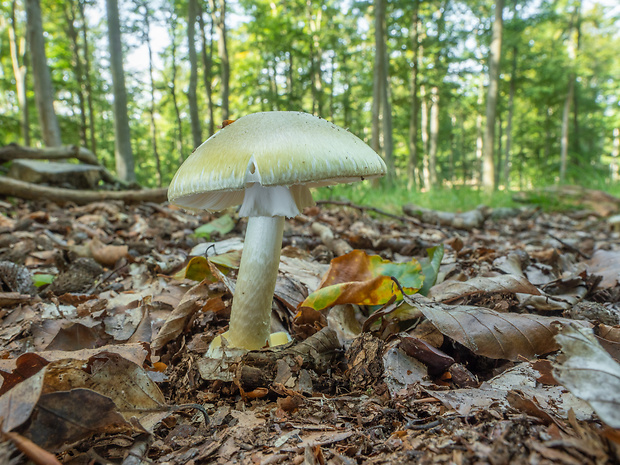
\includegraphics[width=0.35\textwidth]{Images/mucho_z.jpg}} 
    \subfigure[Muchotrávka citronožltá]{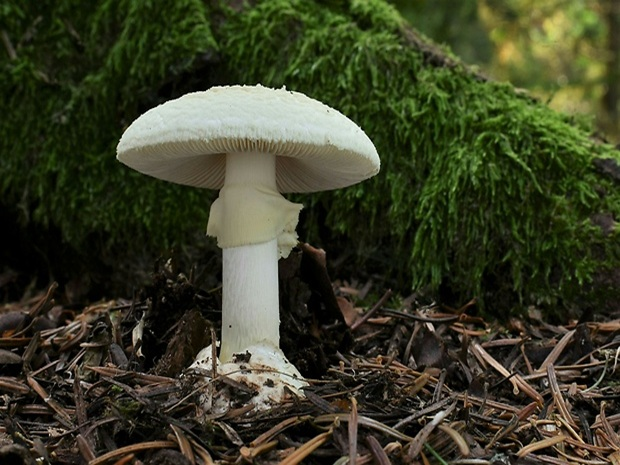
\includegraphics[width=0.35\textwidth]{Images/mucho_c.jpg}} 
    \caption{(a) Autor fotografie Igor Hlavatý \cite{mz}, Malé karpaty (b) Miroslav Valent, Levočské vrchy \cite{mc}}
    \label{fig:foobar}
\end{figure}


\section{Popis použitých modelov}

\subsection{AlexNet}
\IEEEPARstart{}{}je hlboká konvolučná neurónová sieť, ktorá získala pozornosť po víťazstve v súťaži ILSVRC 2012. Architektúra pozostáva z ôsmich vrstiev, z toho päť konvolučných a tri plne prepojené. Využíva nelineárnu aktivačnú funkciu ReLU, max-pooling pre zníženie priestorovej dimenzie a dropout na redukciu pretrénovania. Tréning bol rozdelený medzi dve GPU, čo umožnilo efektívne spracovanie rozsiahlych dát.
\begin{figure}[!htb]
    \centering
    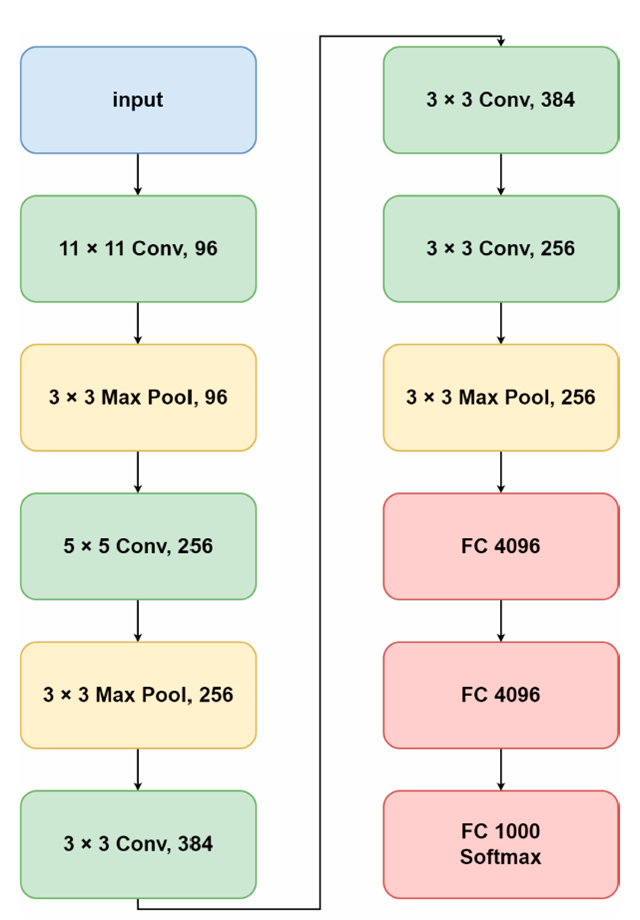
\includegraphics[width=0.35\linewidth]{Images/arch_alexnet.png}
    \caption{Architektúra AlexNet \cite{pc}}
    \label{fig:enter-label}
\end{figure}

\clearpage

\subsection{GoogleNet}
\IEEEPARstart{}{}známa aj ako Inception v1, je hlboká konvolučná neurónová sieť navrhnutá s cieľom znížiť počet parametrov a výpočtov bez straty presnosti. Jej kľúčovou súčasťou je tzv. \textit{Inception modul}, ktorý umožňuje paralelné spracovanie obrazu rôznymi veľkosťami filtrov (1×1, 3×3, 5×5) a poolingom, čím sieť efektívne zachytáva viacero mierok informácie.

Architektúra obsahuje niekoľko po sebe idúcich Inception modulov, pred ktorými sú úvodné konvolučné a pooling vrstvy. Namiesto tradičných plne prepojených vrstiev na konci siete využíva global average pooling, čím výrazne znižuje počet parametrov. Výstupom je softmax klasifikácia na 1000 tried.
\begin{figure}[!htb]
    \centering
    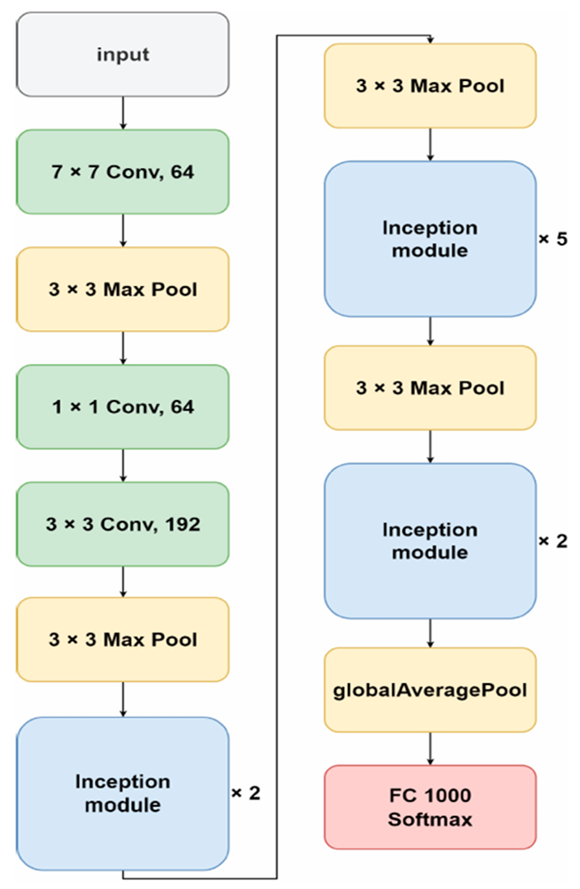
\includegraphics[width=0.4\linewidth]{Images/arch_googlenet.png}
    \caption{Architektúra GoogleNet \cite{pc}}
    \label{fig:enter-label}
\end{figure}

\begin{figure}[!htb]
    \centering
    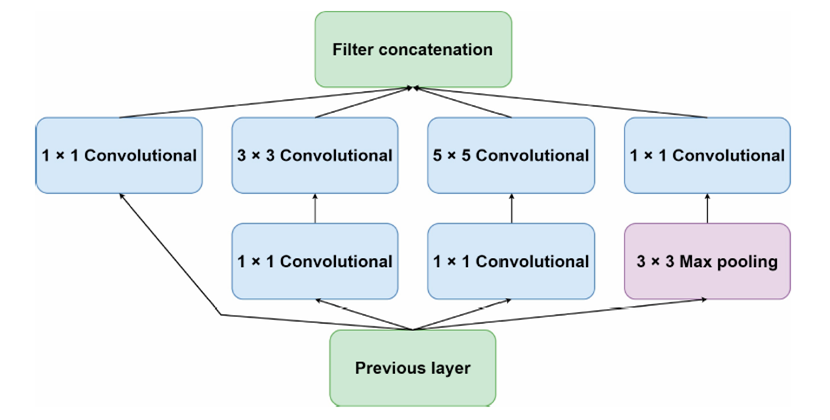
\includegraphics[width=0.65\linewidth]{Images/arch_inceptionmodule.png}
    \caption{Architektúra incepčného modulu \cite{pc}}
    \label{fig:enter-label}
\end{figure}

\newpage
\subsection{ResNet-50}
\IEEEPARstart{}{}je hlboká konvolučná neurónová sieť, ktorá využíva architektúru zvanú \textit{residual learning}. Hlavnou inováciou je zavedenie reziduálnych spojení (tzv. skip connections), ktoré umožňujú priamy prenos informácie naprieč vrstvami a tým efektívnejší tréning veľmi hlbokých sietí.
Architektúra ResNet-50 obsahuje 50 vrstiev a skladá sa z opakujúcich sa \textit{bottleneck} blokov. Každý blok má tri vrstvy: 1×1, 3×3 a opäť 1×1 konvolúciu, pričom prvá a posledná slúžia na redukciu a následné zväčšenie dimenzie. Použitím týchto blokov spolu s reziduálnymi spojeniami sa minimalizuje problém miziaceho gradientu a zlepšuje sa generalizácia modelu.

\begin{figure}[!htb]
    \centering
    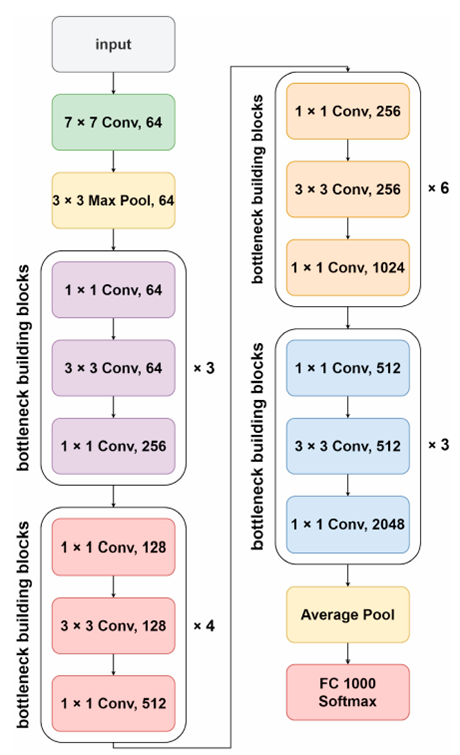
\includegraphics[width=0.45\linewidth]{Images/arch_resnet50.png}
    \caption{Architektúra ResNet-50 \cite{pc}}
    \label{fig:enter-label}
\end{figure}

\newpage
\subsection{Propozovaný model}
\IEEEPARstart{}{} Nový model vytvorený na báze AlexNet-u, 4. a 5. konvolučná vstva bola odstránená a nahradená incepčným modulom z GoogleNet čo by malo teoreticky zvýšiť jeho výkon. 


\begin{figure}[!htb]
    \centering
    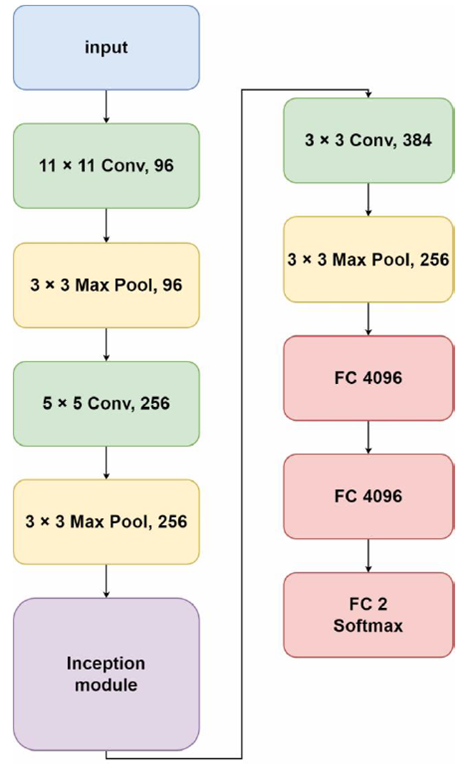
\includegraphics[width=0.45\linewidth]{Images/arch_proposed.png}
    \caption{Architektúra propozovaného modelu \cite{pc}}
    \label{fig:enter-label}
\end{figure}

\newpage
\section{Metodológia}
\subsection{CNN}
Každý z modelov bol upravený, aby sa na nich mohlo uskutočniť pretrénovanie (transfer learning). Dataset 2000 obrázkov bol použitý dvoma spôsobmi :
\begin{enumerate}[label=\Alph*]
  \item Použitý metódou k-fold cross validation na získanie presnej hodnoty priemernej trénovaciej presnosti. 
  \item Vytvorenie trénovacej a testovacej vzorky v pomere 9:1, tento train-test set bol rovnaký pre všetky CNN a bol použítý na získanie výsledných metrík modelov.
\end{enumerate}
\vspace{10pt}
\subsubsection{k-fold cross validation}
Princíp fungovania validačnej metódy je nasledovný :
\begin{enumerate}
  \item Dataset je rozdelený na k počet skupiniek (folds)
  \item Jedna z k skupiniek je vybraná ako test set a zvyšok (k - 1) je použitý ako train set
  \item Po trénovaní a testovaní modelu získame metriku, ktorá nás zaujíma pre iteráciu k
  \item Proces sa opakuje dokiaľ sa všetky k skupinky nevystriedali byť test set-om
  \item Výsledkom metódy je priemer metriky všetkých k iterácií
\end{enumerate}
\vspace{10pt}
Táto metóda slúži na to, aby výsledná metrika, ktorú sa snažíme nájsť, nebola nijak ovplyvnená len variáciou v test set-e. V našom prípade bol dataset rozdelený na 10 k skupiniek (rôzne pre každý model), každá s počtom 200 obrázkov. Nami hľadaná metrika bola priemerná testovacia presnosť, kde pri trénovaní slúžil k-tý test set ako validation set. Každý model bol teda trénovaný 10-krát na rôznych variáciách train a validation set-u na získanie výslednej priemernej trénovacej presnosti.  

\subsection{RCNN}
Každý z modelov bol upravený na to, aby mohol byť použitý ako súčasť RCNN. Pôvodný súbor dataset-u síce obsahoval priečinok rcnn s obrázkami pretvarovanými na veľkosť 300 X 300 X 3 pixelov, ale samotné anotácie obrázkov nutné pre trénovanie RCNN neboli poskytnuté. To znamenalo, že sme museli 2000 obrázkov anotovať sami, urobili sme to manuálne pomocou {\it MatLab Image Labeler}. Tento dataset bol potom rozdelený na train a test set v mierke 9:1, čiže 1800 obrázkov s anotáciami a 200 bez.

\vspace{10pt}
\subsubsection{RCNN (Region Convolutional Neural Network)}
Tradičný CNN síce vie klasifikovať objekt, ale nijak neukazuje v ktorej časti obrázku sa nachádza. RCNN vie nielen klasifikovať objekt ale aj nakreslí takzvaný "bounding box" okolo oblasti kde sa objekt (podľa modelu) nachádza. Funguje v 4 krokoch :
\begin{enumerate}
  \item Z obrázka sa extraktuje 2000 "region proposals" ktoré sa potom pretvarujú na rovnakú veľkosť a použijú sa ako vstup do CNN 
  \item Pomocou CNN sú extraktované prvky pre každý region proposal
  \item Extraktované prvky sú použité na klasifikáciu region proposals pomocou algoritmu SVM (Support Vector Machine)
  \item Bounding box-y sú vytvorené okolo objektov
\end{enumerate}

\begin{figure}[!htb]
    \centering
    \subfigure[]{\includegraphics[width=0.3\textwidth]{Images/RCNN_Example1.png}} 
    \subfigure[]{\includegraphics[width=0.3\textwidth]{Images/RCNN_Example2.png}}
    \subfigure[]{\includegraphics[width=0.3\textwidth]{Images/RCNN_Example3.png}} 
    \caption{Príklady klasifikácie pomocou RCNN}
    \label{fig:foobar}
\end{figure}

\newpage
\section{Implementačné rozdiely}
\IEEEPARstart{P}{ôvodný} článok sme sa snažili replikovať čo najlepšie sme mohli, nič sme úmyselne neurobili inak ako v pôvodnom vypracovaní, všetky implementačné rozdiely (ktoré sú nami známe) vznikli len základe nedostatku informácií z článku a technických dôvodov.

\subsection{Vytvorenie propozovaného modelu}
V článku je síce popísaná štruktúra propozovaného modelu ale neni presne dané, z ktorej časti GoogleNet bol vybraný incepčný modul ktorý sa v ňom nachádza alebo ako boli vrstvy AlexNet zmenené na kompabilitu s incepčným modulom. Mi sme propozovaný model vytvorili nasledovným spôsobom.

\begin{enumerate}
  \item AlexNet bol rozdelený na dve časti odstránením 4. a 5. konvolučnej vrsty
  \item K prvej časti bol pripojený 2. incepčný modul 1. incepčného bloku GoogleNet
  \item Druhá časť bola pripojená na koniec incepčného modulu
  \item Prvé dve vrstvy druhej časti boli modifikované aby boli kompatibilné s incepčným modulom
\end{enumerate}

Je možné že model v pôvodnom článku bol vytvorený iným spôsobom.

\subsection{Neznámy optimalizátor}
V článku neni spomenuté aký optimalizátor bol použitý pri trénovaní modelov. Pomocou experimentácie sme došli k tomu že to bol s najväčšou pravdepodobnosťou SGDM.

\subsection{Anotovanie dataset-u pre RCNN}
V článku neni nijak popísané akým spôsobom boli obrázky anotované pre trénovanie RCNN či manuálne alebo pomocou algoritmu. Mi sme dataset anotovali manuálne, čo je možno iný spôsob ako ktorí použili autori pri pôvodnom vypracovaní a môže to mať vplyv na výsledky.

\subsection{MatLab verzia}
V článku bol použitý MatLab R2021b, čo mi sme použili MatLab R2024b.

\section{Deep Dreams}
\IEEEPARstart{}{}je technika vizualizácie, ktorú vyvinula spoločnosť Google na interpretáciu a pochopenie toho, čo sa neurónové siete naučili. Využíva spätnú propagáciu (backpropagation), ale namiesto úpravy váh siete upravuje samotný vstupný obrázok tak, aby maximalizoval aktiváciu určitých neurónov. Výsledkom sú „snové“ obrázky s psychedelickými vzormi a opakujúcimi sa motívmi, ktoré odrážajú vnútorné reprezentácie siete.

\begin{figure}[!htb]
    \centering
    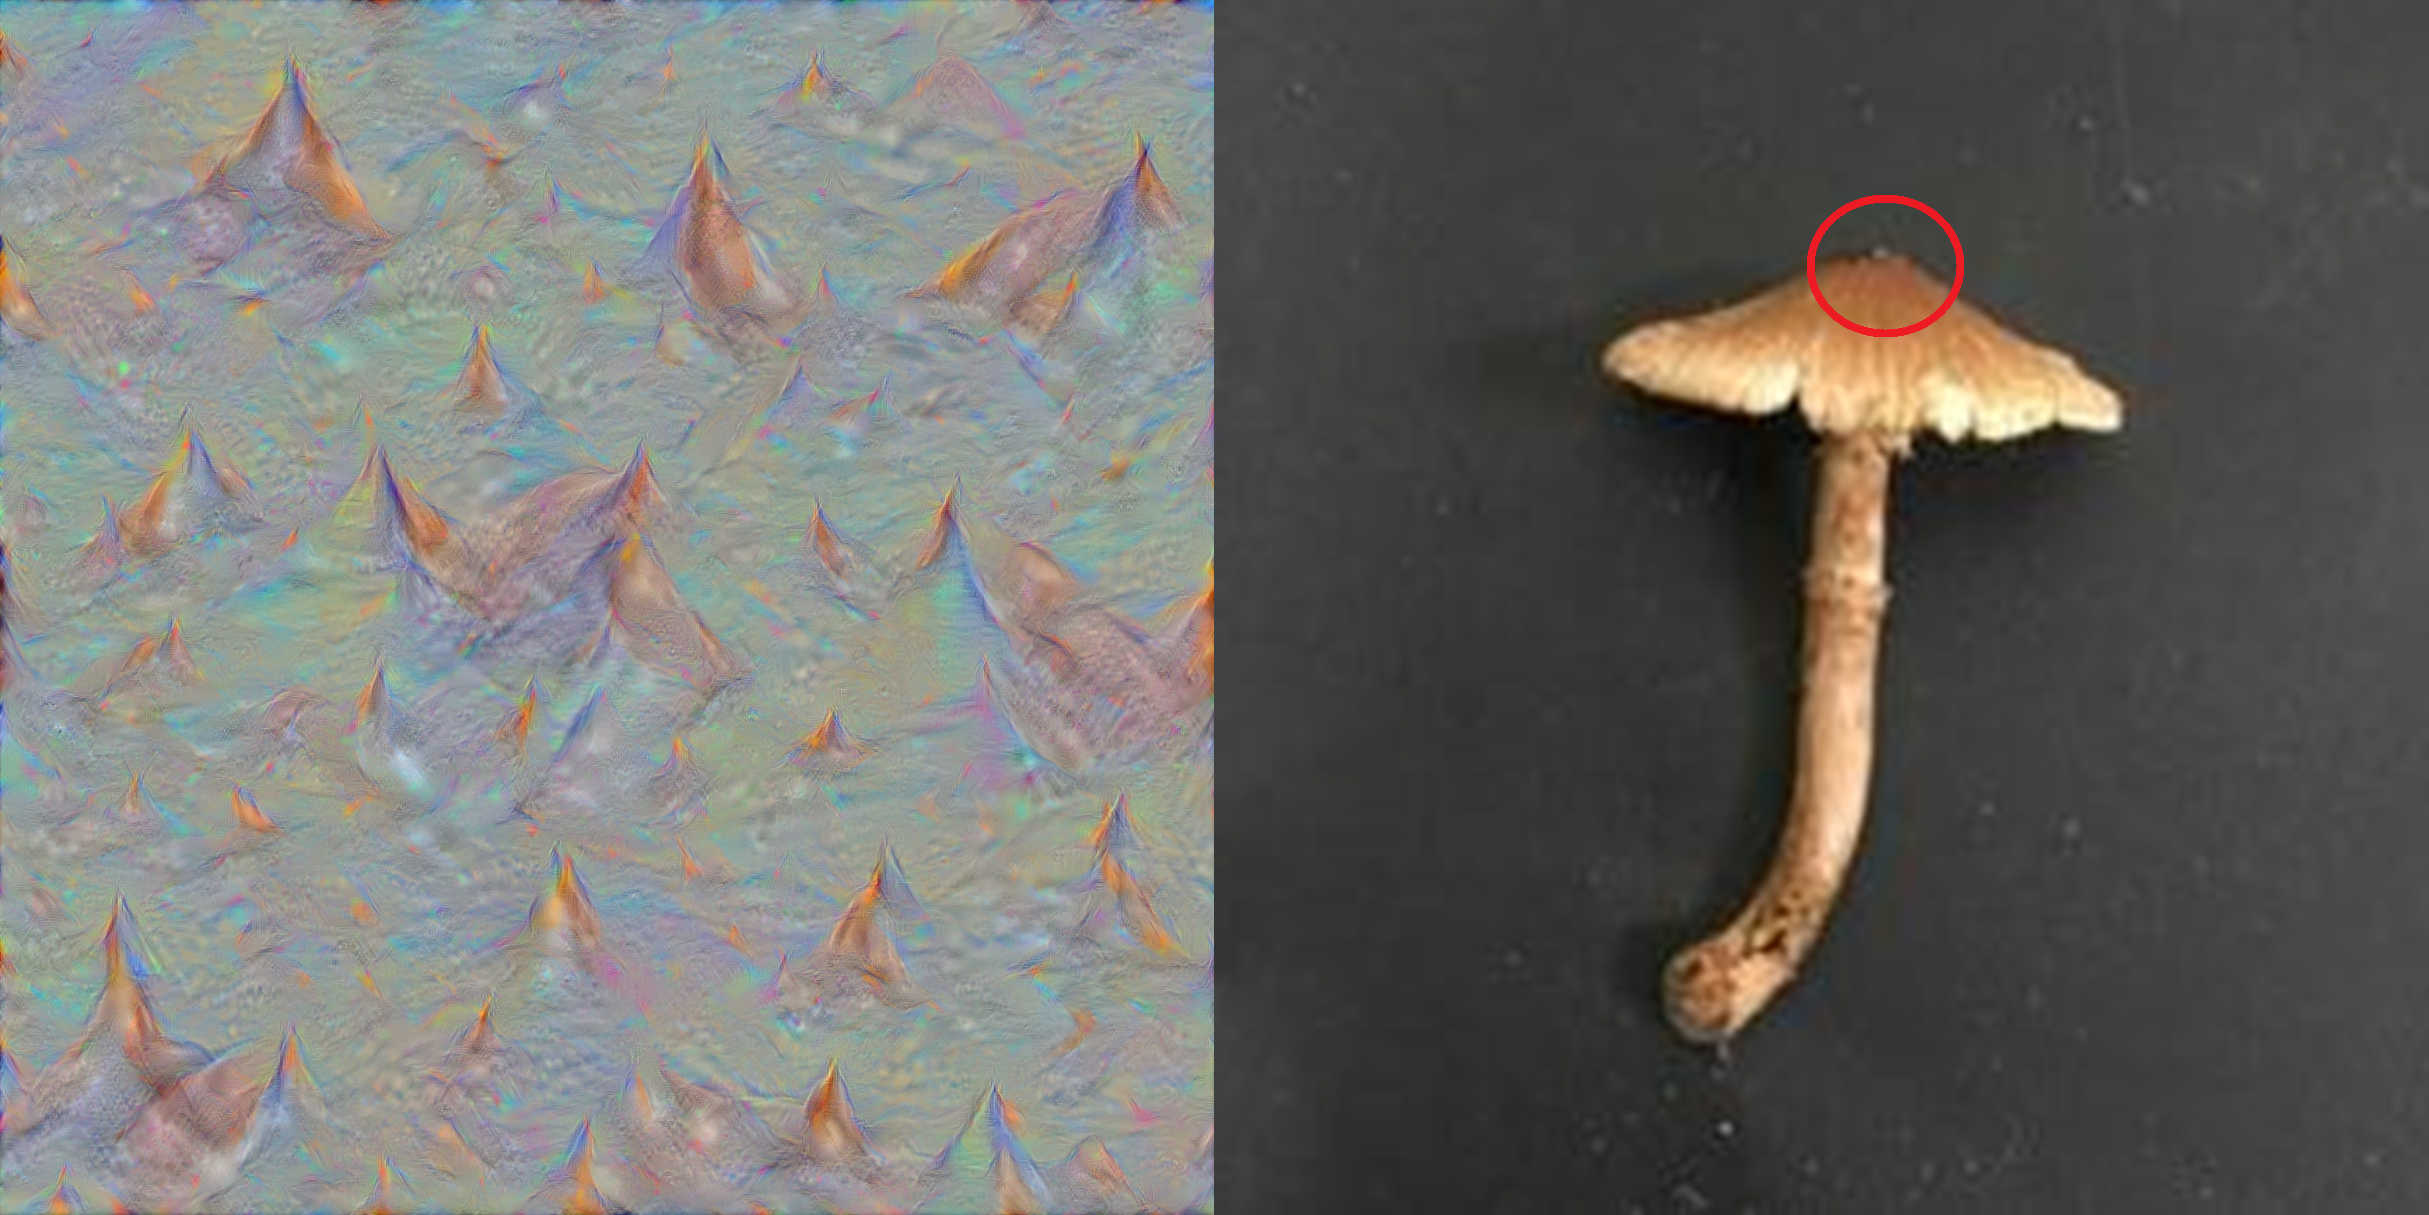
\includegraphics[width=0.6\linewidth]{Images/dp_example.png}
    \caption{Príklad deep dream obrázka}
    \label{fig:enter-label}
\end{figure}

\newpage

\section{Výsledky}
\IEEEPARstart{V}{šetky} výsledky boli získané pomocou MatLab R2024b, na počítači s procesorom Intel Core i5 10400F, RAM pamäťou 16 GB a grafickou kartou NVIDIA RTX 3070. Pôvodný článok použil MatLab R2021b na počítači s Intel Core i5 12600, RAM pamäťou 12 GB a grafickou kartou NVIDIA RTX 3060. Čiže o 2 generácie a 2 rady lepší procesor ale o radu horšiu grafickú kartu.

\subsection{CNN - Priemerná trénovacia presnosť}
Pre každý model boli použité rovnaké hyper-parametre :
\begin{enumerate}
  \item Optimalizátor = SGDM
  \item Learning rate = 0.001
  \item Počet epoch = 10
  \item Batch size = 40
\end{enumerate}

\subsubsection{AlexNet}
AlexNet dosiahol priemernú trénovaciu presnosť s hodnotou 98.88 \%, pričom najlepšia k iterácia (k=8) dosiahla presnosť až 99.50 \%, trénovací graf tejto iterácie je zobrazený nasledovne.

\begin{figure}[!htb]
    \centering
    \subfigure[]{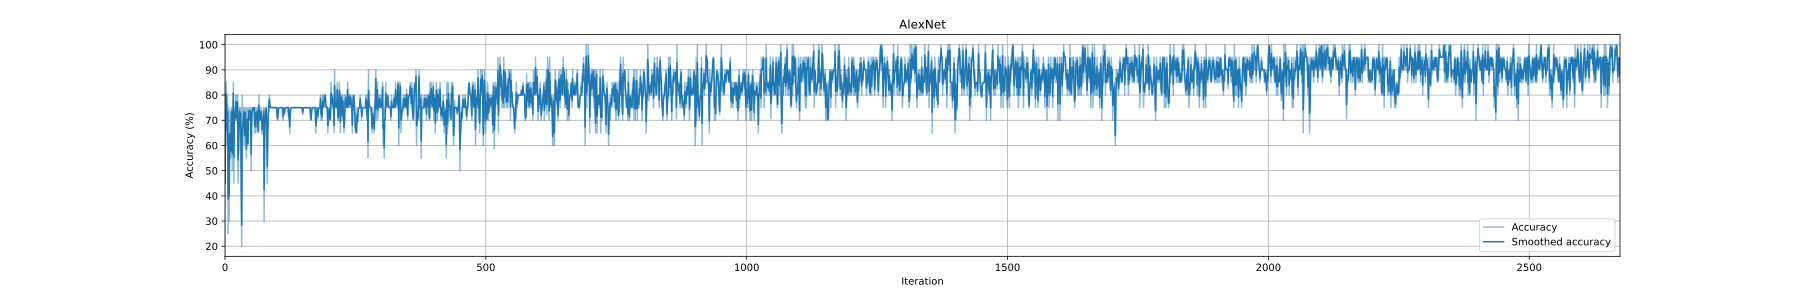
\includegraphics[width=1\textwidth]{Images/AlexNet_TrainGraphAcc.png}} 
    \subfigure[]{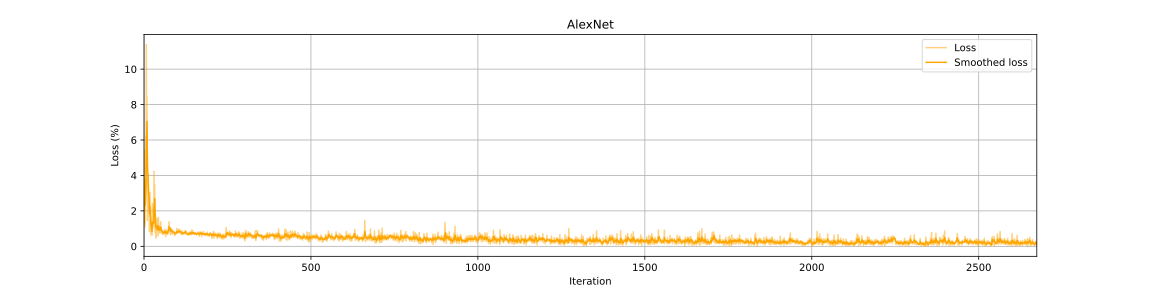
\includegraphics[width=1\textwidth]{Images/AlexNet_TrainGraphLoss.png}}
    \caption{(a) Trénovací graf presnosti AlexNet (b) Trénovací graf chyby AlexNet}
    \label{fig:foobar}
\end{figure}

\subsubsection{GoogleNet}
GoogleNet dosiahol priemernú trénovaciu presnosť s hodnotou 99.70 \%, pričom najlepšia k iterácia (k=3) dosiahla presnosť až 100 \%, trénovací graf tejto iterácie je zobrazený nasledovne.

\newpage

\begin{figure}[!htb]
    \centering
    \subfigure[]{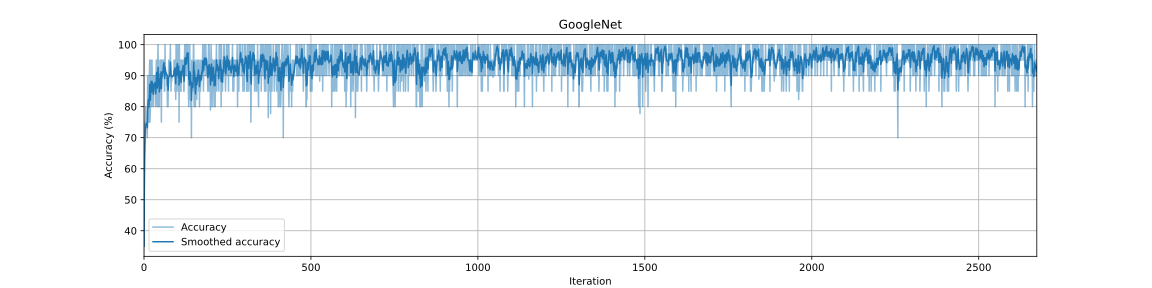
\includegraphics[width=0.7\textwidth]{Images/GoogleNet_TrainGraphAcc.png}} 
    \subfigure[]{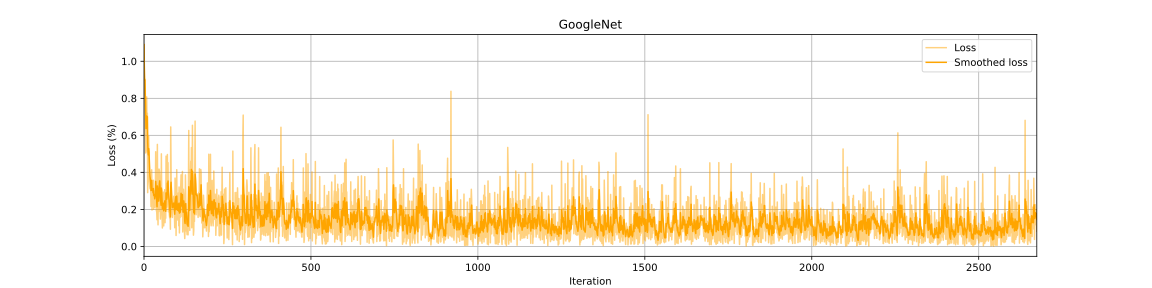
\includegraphics[width=0.7\textwidth]{Images/GoogleNet_TrainGraphLoss.png}}
    \caption{(a) Trénovací graf presnosti GoogleNet (b) Trénovací graf chyby GoogleNet} 
    \label{fig:foobar}
\end{figure}

\subsubsection{ResNet50}
ResNet50 dosiahol priemernú trénovaciu presnosť s hodnotou 99.88 \%, pričom najlepšia k iterácia (k=1) dosiahla presnosť až 100 \%, trénovací graf tejto iterácie je zobrazený nasledovne.

\begin{figure}[!htb]
    \centering
    \subfigure[]{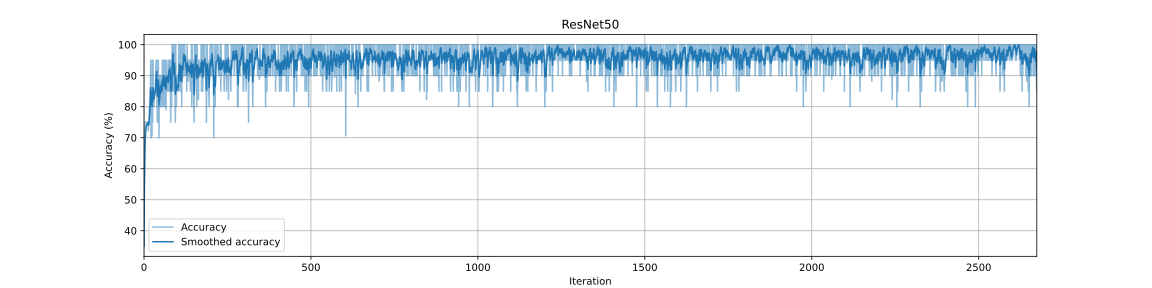
\includegraphics[width=0.65\textwidth]{Images/ResNet50_TrainGraphAcc.png}} 
    \subfigure[]{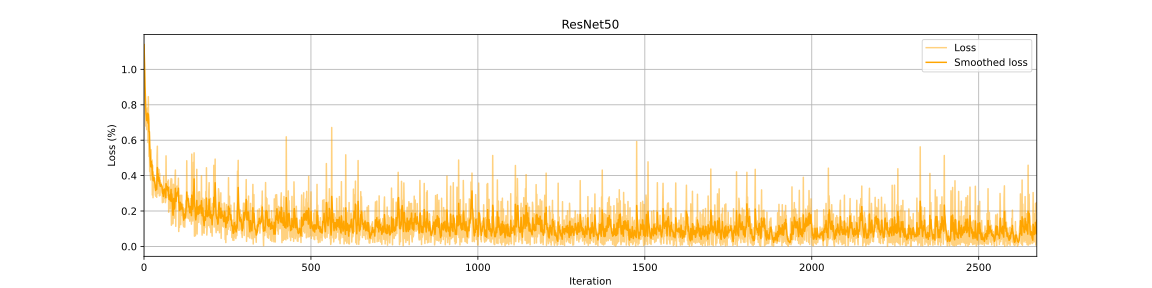
\includegraphics[width=0.65\textwidth]{Images/ResNet50_TrainGraphLoss.png}}
    \caption{(a) Trénovací graf presnosti ResNet50 (b) Trénovací graf chyby ResNet50} 
    \label{fig:foobar}
\end{figure}

\subsubsection{ArticleNet (Propozovaný model)}
 Propozovaný model (nami nazvaný ArticleNet) dosiahol priemernú trénovaciu presnosť s hodnotou 92.53 \%, pričom najlepšia k iterácia (k=4) dosiahla presnosť až 96.50 \%, trénovací graf tejto iterácie je zobrazený nasledovne.

\begin{figure}[!htb]
    \centering
    \subfigure[]{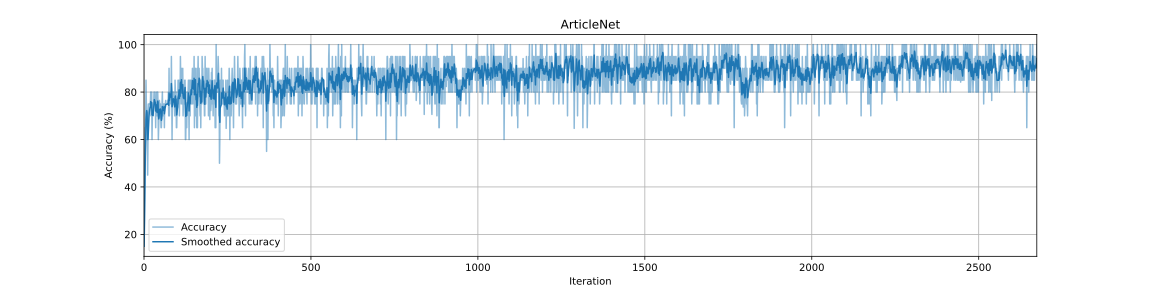
\includegraphics[width=0.7\textwidth]{Images/ArticleNet_TrainGraphAcc.png}} 
    \subfigure[]{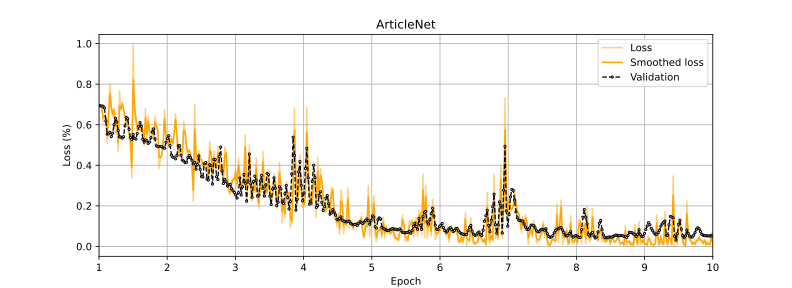
\includegraphics[width=0.7\textwidth]{Images/ArticleNet_TrainGraphLoss.png}}
    \caption{(a) Trénovací graf presnosti propozovaného modelu (b) Trénovací graf chyby propozovaného modelu} 
    \label{fig:foobar}
\end{figure}

\begin{figure}[!htb]
    \centering
    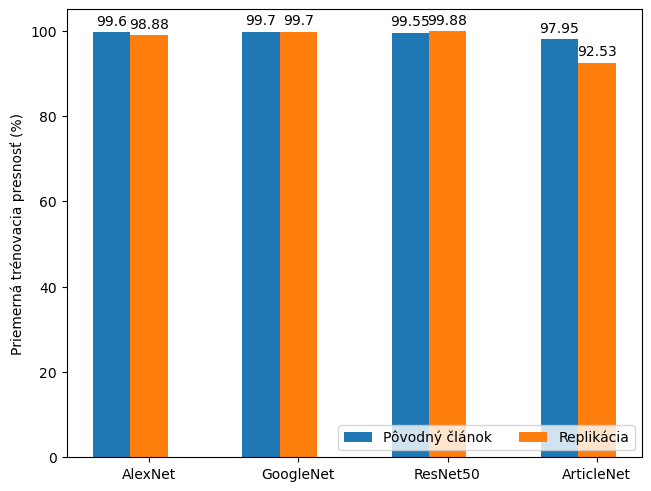
\includegraphics[width=0.6\linewidth]{Images/c_vs_rep.png}
    \caption{Porovnanie priemernej trénovaciej presnosti z článku oproti výsledkom získaných z replikácie}
    \label{fig:enter-label}
\end{figure}

S výnimkou propozovaného modelu (ArticleNet), výsledky replikácie sú v rozsahu $\pm 0.75\%$ od pôvodného článku. Rozdiel 5.42 \% čo sa týka propozovaného modelu je s najväčšou pravdepodobnosťou dôsledok spomenutého implementačného rozdielu A, nedostatok informácií o jeho vytvorení.

\subsection{CNN - Výsledné metriky}

Pre každý model boli použité rovnaké hyper-parametre :
\begin{enumerate}
  \item Optimalizátor = SGDM
  \item Learning rate = 0.001
  \item Počet epoch = 10
  \item Batch size = 40
\end{enumerate}

\vspace{10pt}
Nasledujúca tabuľka popisuje výsledky získané našou replikáciou, hodnoty v zátvorkách určujú o koľko sa hodnota zvýšila rešpektívne znížila oproti hodnote z pôvodného článku.

\captionof{table}{CNN Výsledky replikácie oproti výsledkom z článku}
\begin{center}
{\renewcommand{\arraystretch}{1.5}
\begin{tabular}{|c|ccccc}
\hline
Model & Accuracy & Precision & Recall & F1 & Time \\                            
\hline          

GoogleNet & 
100.00 \textcolor{green}{(+0.50)} & 
100.00 \textcolor{green}{(+0.65)} & 
100.00 \textcolor{gray}{(0.00)} & 
100.00 \textcolor{green}{(+0.03)} & 
1min 31s \textcolor{red}{-(49.00s)} \\

ResNet50 & 
99.50 \textcolor{gray}{(0.00)} & 
99.33 \textcolor{gray}{(0.00)} & 
100.00 \textcolor{gray}{(0.00)} & 
99.66 \textcolor{gray}{(0.00)} & 
3min 13s \textcolor{red}{(-2min 37.00s)} \\

AlexNet & 
99.50 \textcolor{green}{(+0.50)} & 
99.33 \textcolor{green}{(+0.72)} & 
100.00 \textcolor{gray}{(0.00)} & 
99.66 \textcolor{green}{(+0.36)} & 
45s \textcolor{red}{-(57.00s)} \\

ArticleNet & 
99.00 \textcolor{green}{(+0.50)} & 
99.33 \textcolor{red}{(-0.06)} & 
99.33 \textcolor{green}{(+0.54)} & 
99.33 \textcolor{green}{(+0.24)} & 
40s \textcolor{red}{(-30.00s)}

\end{tabular}}
\end{center}

\vspace{10pt}
Jak môžeme vidieť v tabuľke, hodnoty replikácie sú všetky v rozsahu $\pm 1\%$ a v prípade F1 skóre dokonca až len $\pm 0.5\%$ od pôvodného článku čo indikuje že replikáciu sme urobili úspešne. Trénovacie časy modelov sú samozrejme nižšie z dôvodu použitia lepšej grafickej karty.

\begin{figure}[!htb]
    \centering
    \subfigure[GoogleNet]{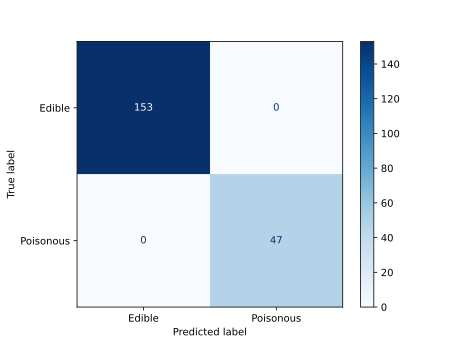
\includegraphics[width=0.42\textwidth]{Images/GoogleNet_ConfusionMatrix.png}} 
    \subfigure[ResNet50]{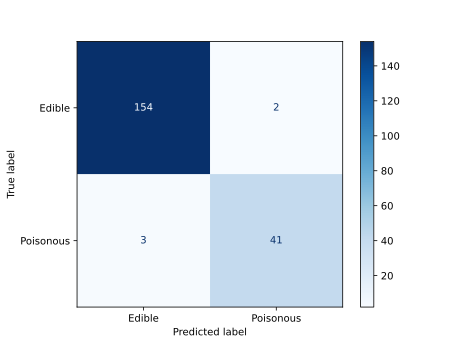
\includegraphics[width=0.42\textwidth]{Images/ResNet50_ConfusionMatrix.png}} 
    \subfigure[AlexNet]{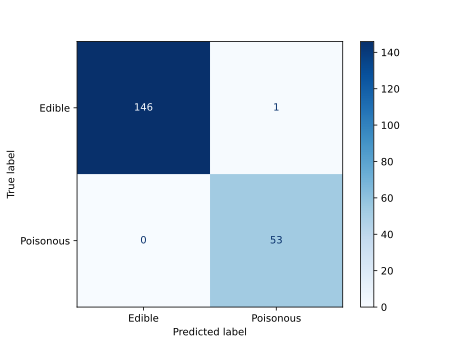
\includegraphics[width=0.42\textwidth]{Images/AlexNet_ConfusionMatrix.png}} 
    \subfigure[ArticleNet]{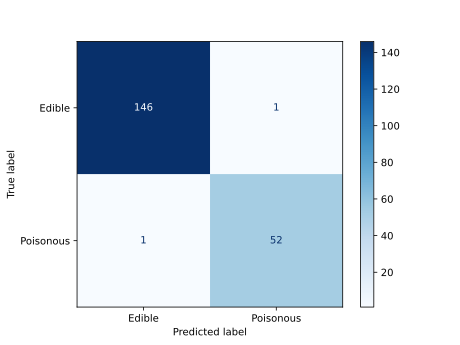
\includegraphics[width=0.42\textwidth]{Images/ArticleNet_ConfusionMatrix.png}} 
    \caption{CNN Confúzne matice modelov}
    \label{fig:foobar}
\end{figure}

\subsection{CNN Deep Dreams}
\subsubsection{AlexNet}
AlexNet dosahoval najvyššiu aktivačnú metriku, čiže obrázky sú veľmi detailné.
\begin{figure}[!htb]
    \centering
    \subfigure[]{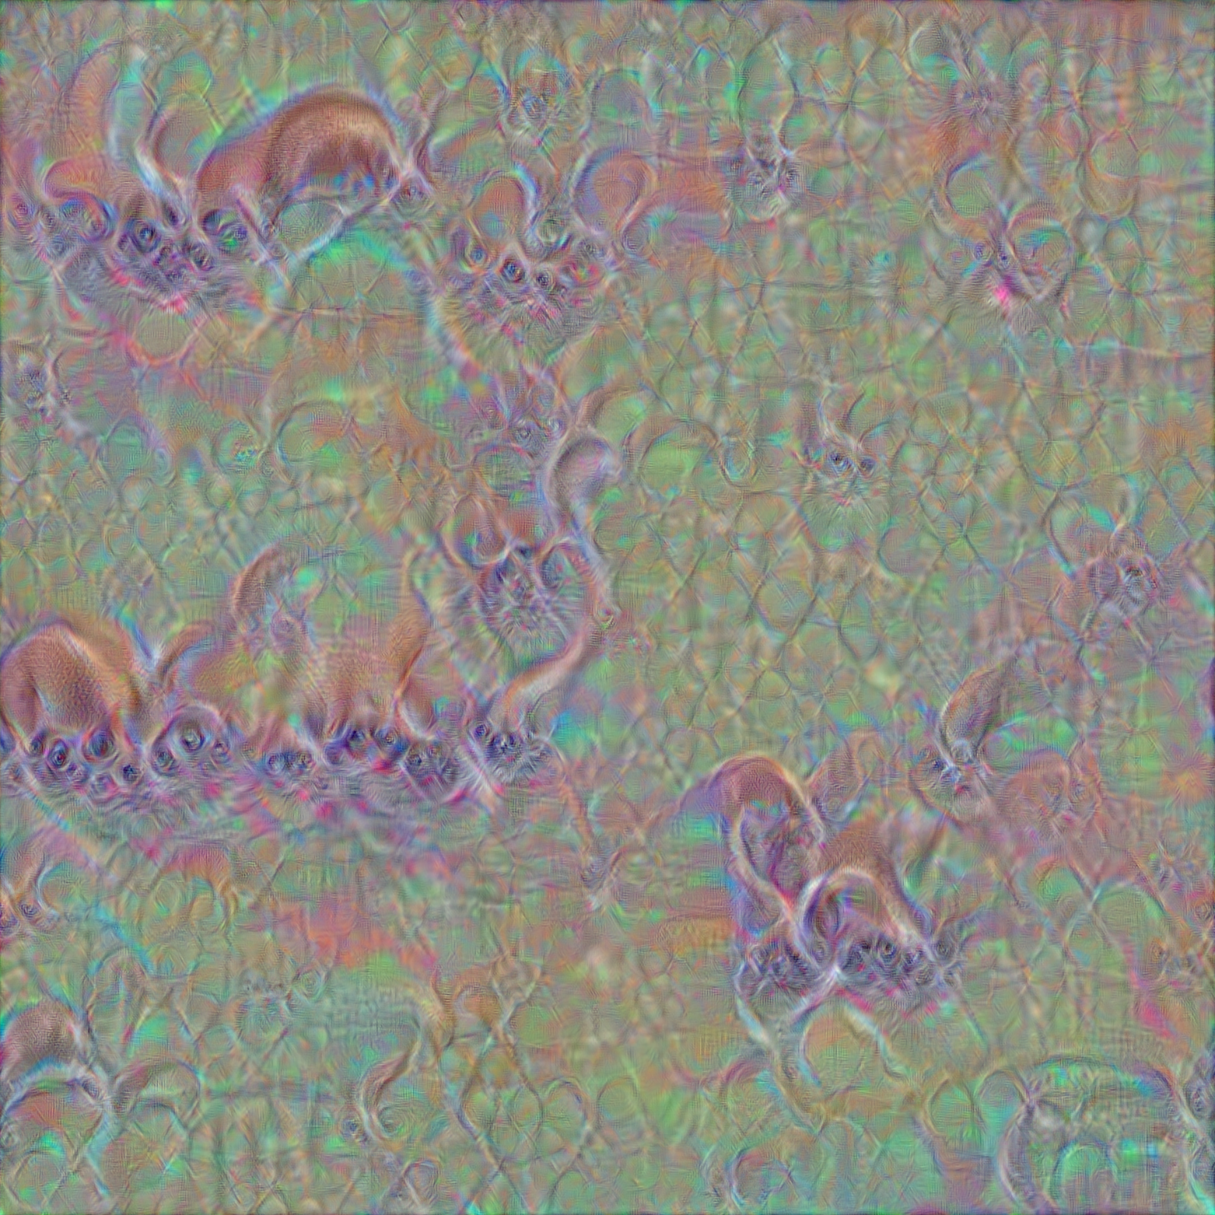
\includegraphics[width=0.22\textwidth]{Images/AlexDP1.png}} 
    \subfigure[]{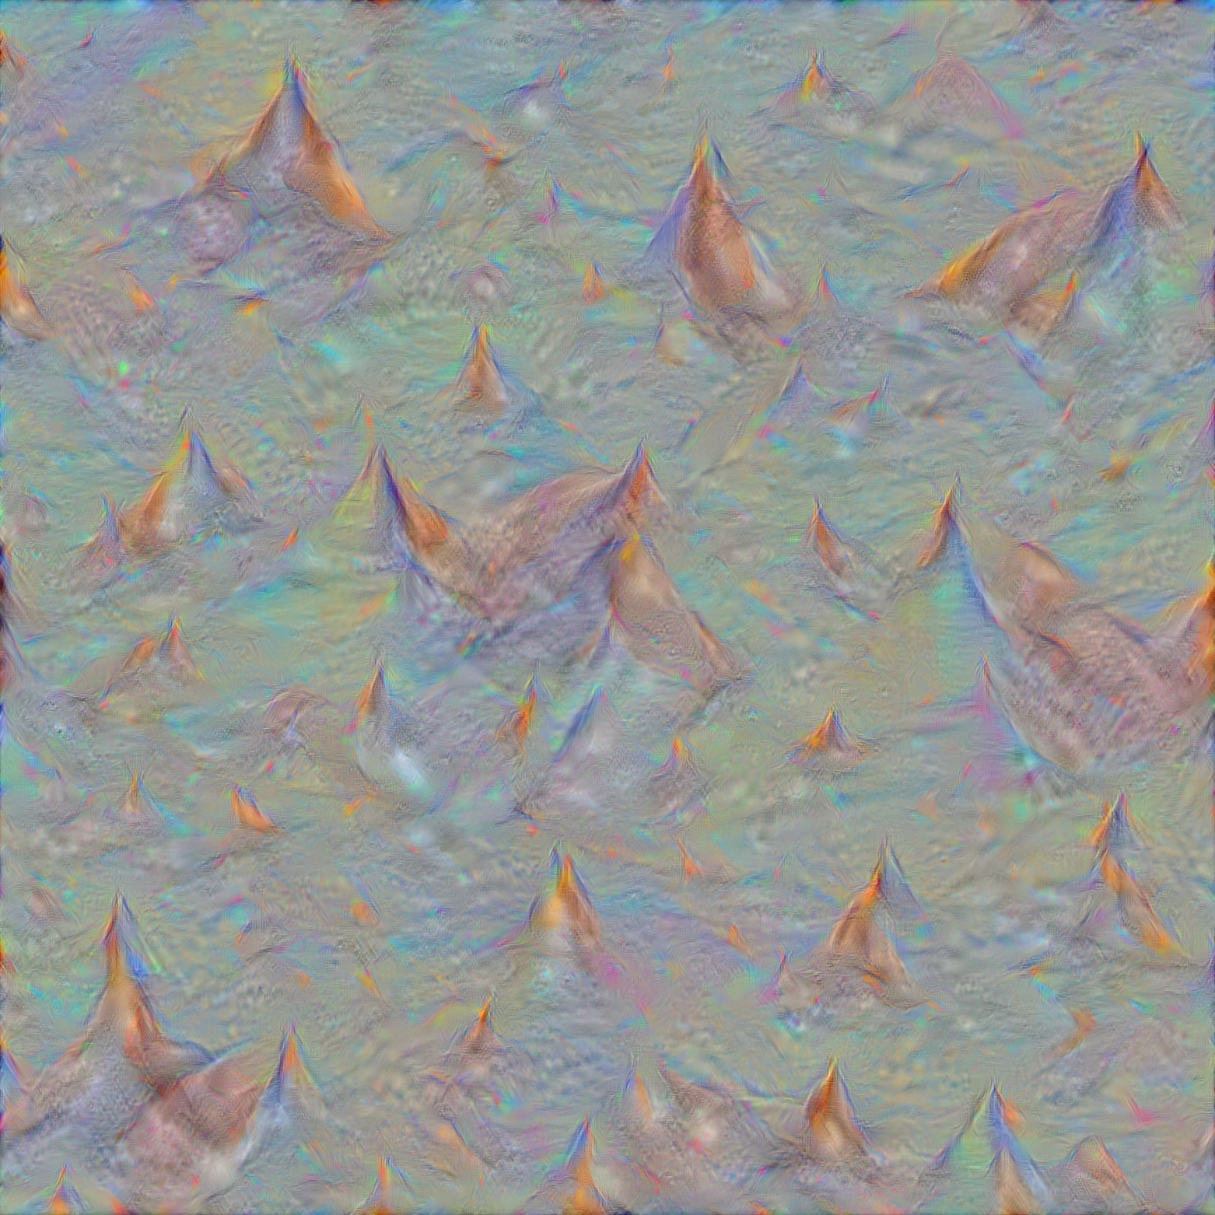
\includegraphics[width=0.22\textwidth]{Images/AlexDP2.png}}
    \subfigure[]{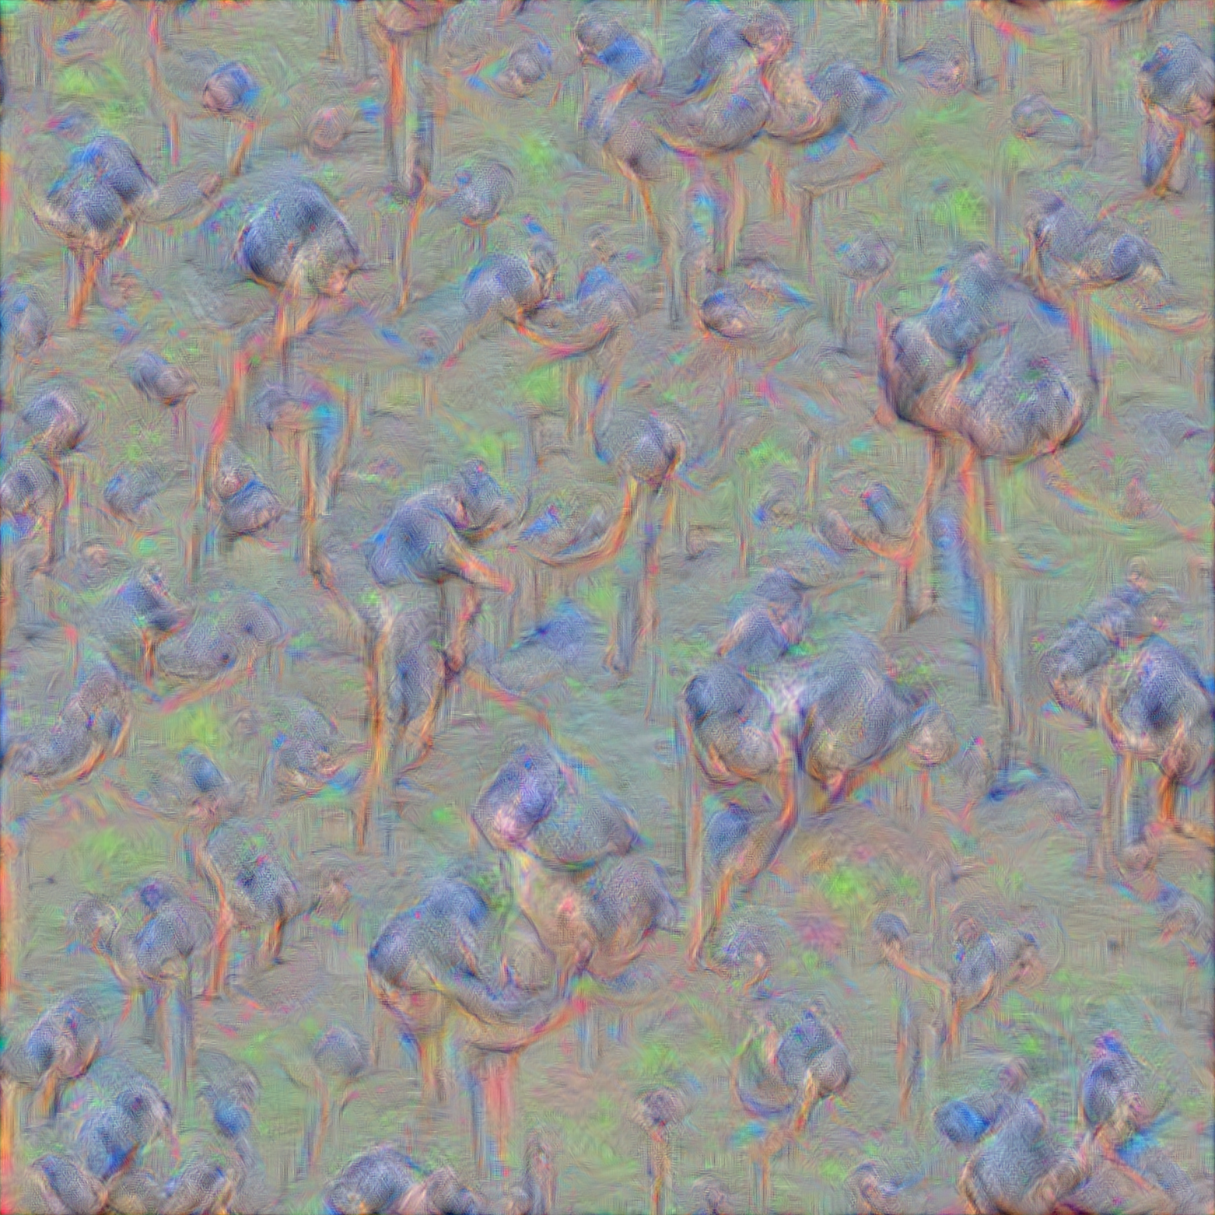
\includegraphics[width=0.22\textwidth]{Images/AlexDP3.png}} 
    \caption{Deep dream obrázky z fc7 vrsty AlexNet-u}
    \label{fig:foobar}
\end{figure}

\subsubsection{GoogleNet} \textcolor{white}{*}
\begin{figure}[!htb]
    \centering
    \subfigure[]{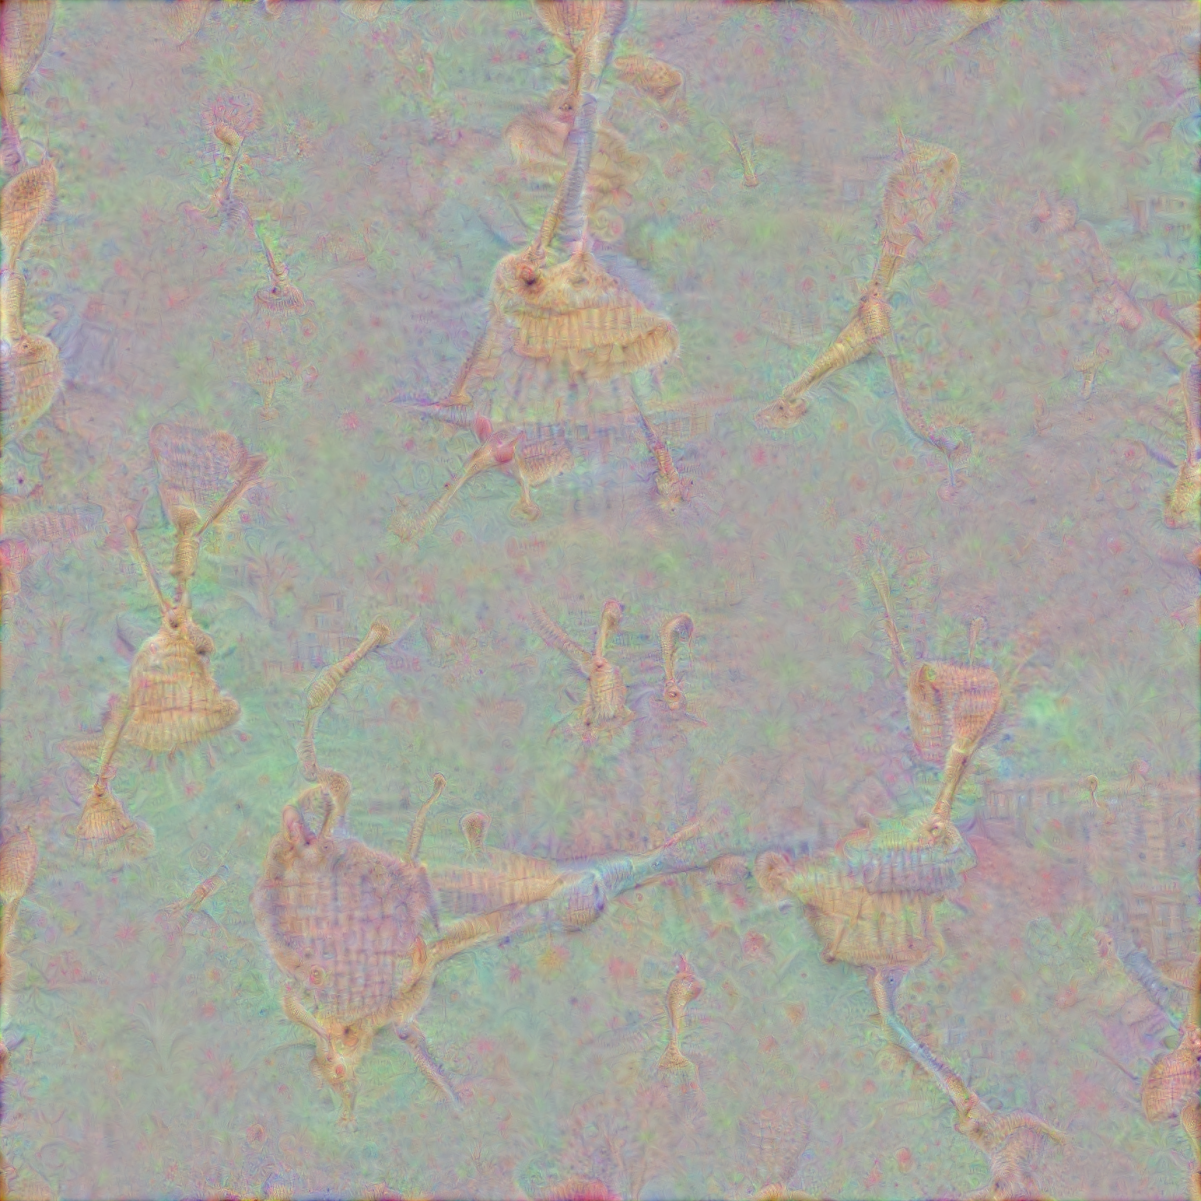
\includegraphics[width=0.18\textwidth]{Images/GoogleDP1.png}} 
    \subfigure[]{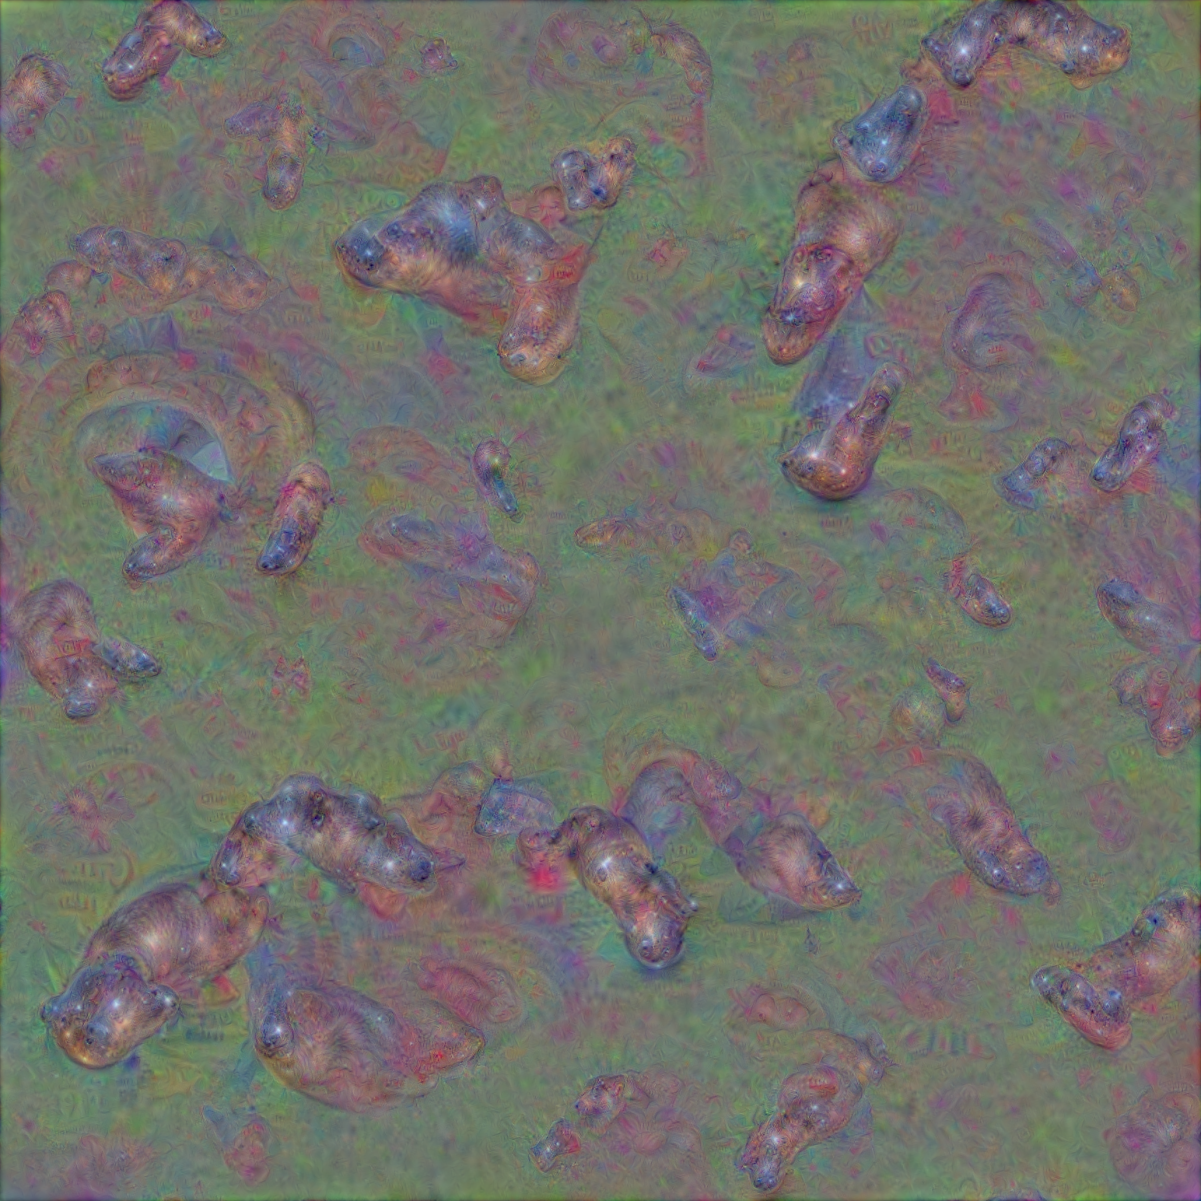
\includegraphics[width=0.18\textwidth]{Images/GoogleDP2.png}}
    \caption{Deep dream obrázky z loss3-classifier vrsty GoogleNet-u}
    \label{fig:foobar}
\end{figure}

\subsubsection{ResNet50} \textcolor{white}{*}
\begin{figure}[!htb]
    \centering
    \subfigure[]{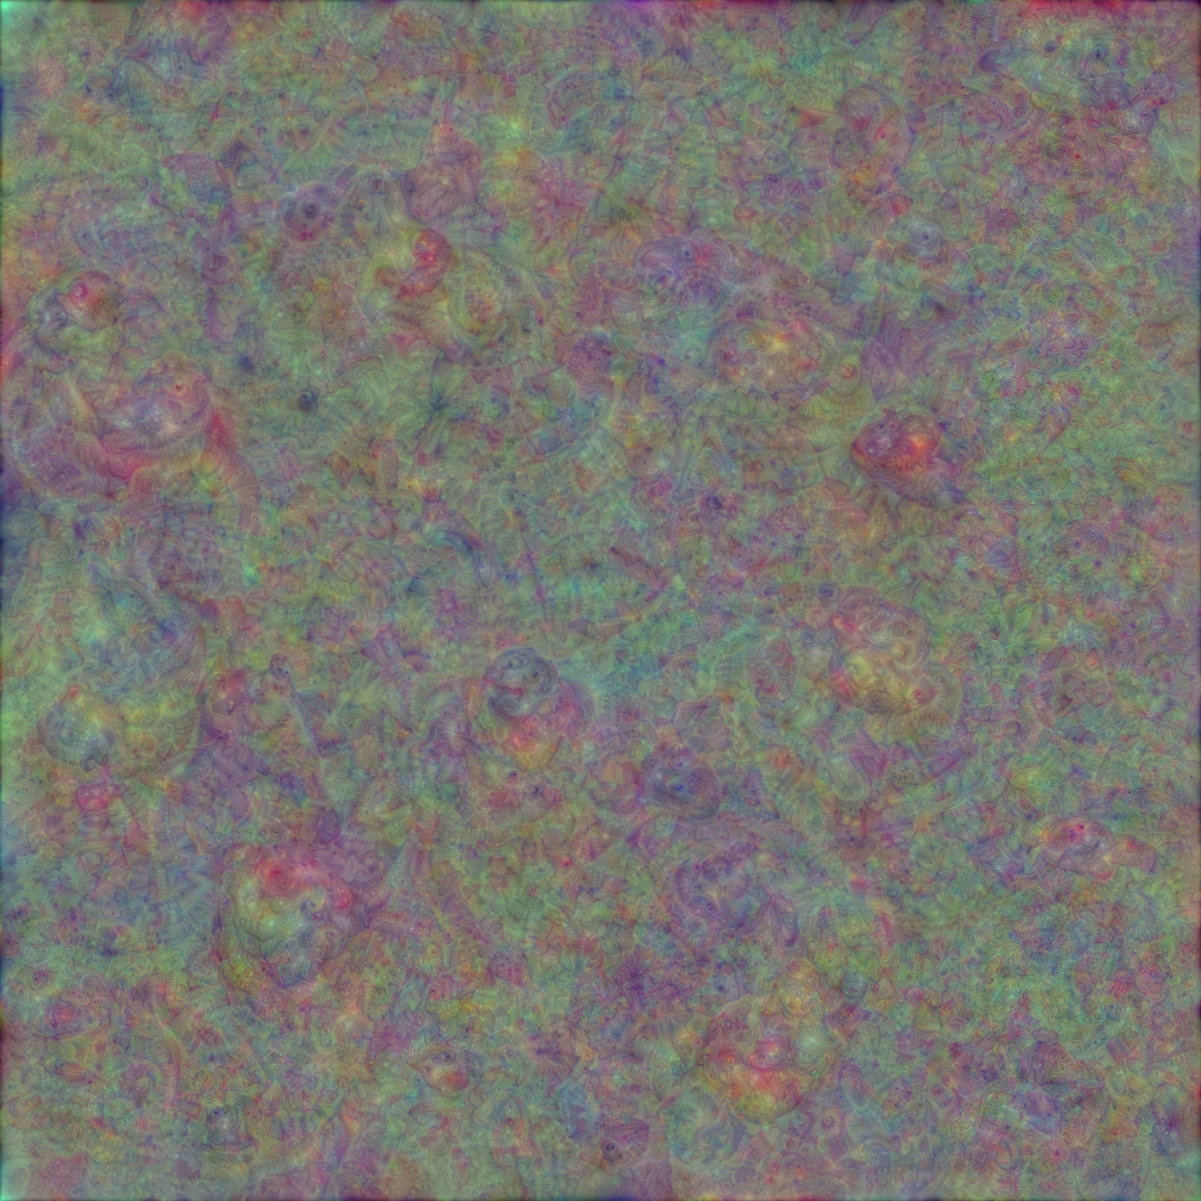
\includegraphics[width=0.16\textwidth]{Images/ResDP1.png}} 
    \subfigure[]{
\includegraphics[width=0.16\textwidth]{Images/ResDP2.png}}
    \caption{Deep dream obrázky z fc1000 vrsty ResNet50}
    \label{fig:foobar}
\end{figure}

\subsubsection{ArticleNet} \textcolor{white}{*}
\begin{figure}[!htb]
    \centering
    \subfigure[]{
\includegraphics[width=0.16\textwidth]{Images/ArticleDP1.png}} 
    \subfigure[]{
\includegraphics[width=0.16\textwidth]{Images/ArticleDP2.png}}
    \subfigure[]{
\includegraphics[width=0.16\textwidth]{Images/ArticleDP3.png}}
    \caption{Deep dream obrázky z fc7 vrsty ArticleNet-u (propozovaného modelu)}
    \label{fig:foobar}
\end{figure}

\subsection{RCNN}

Pre každý model boli použité rovnaké hyper-parametre :
\begin{enumerate}
  \item Optimalizátor = SGDM
  \item Learning rate = 0.001
  \item Počet epoch = 1
  \item Batch size = 20
\end{enumerate}

\vspace{10pt}
Nasledujúca tabuľka popisuje výsledky získané našou replikáciou, hodnoty v zátvorkách určujú o koľko sa hodnota zvýšila rešpektívne znížila oproti hodnote z pôvodného článku.

\captionof{table}{RCNN Výsledky replikácie oproti výsledkom z článku}
\begin{center}
{\renewcommand{\arraystretch}{1.5}
\begin{tabular}{|c|ccccc}
\hline
Model & Accuracy & Precision & Recall & F1 & Time \\                            
\hline          

GoogleNet & 
97.50 \textcolor{green}{(+1.00)} & 
98.04 \textcolor{red}{(-1.26)} & 
98.68 \textcolor{green}{(+2.76)} & 
98.36 \textcolor{green}{(+0.78)} & 
5min 40s \textcolor{red}{(-1min 48.00s)} \\

ResNet50 & 
96.00 \textcolor{red}{(-0.50)} & 
95.42 \textcolor{red}{(-4.58)} & 
99.32 \textcolor{green}{(+4.08)} & 
97.33 \textcolor{red}{(-0.23)} & 
11min 51s \textcolor{red}{(-1min 53.00s)} \\

ArticleNet & 
95.00 \textcolor{red}{(-0.50)} & 
94.77 \textcolor{green}{(+0.18)} & 
98.64 \textcolor{red}{(-0.65)} & 
96.67 \textcolor{red}{(-0.22)} & 
2min 39s \textcolor{red}{(-1min 58.00s)} \\

AlexNet & 
95.00 \textcolor{gray}{(0.00)} & 
100.00 \textcolor{green}{(+2.76)} & 
93.87 \textcolor{red}{(-2.05)} & 
96.84 \textcolor{green}{(+0.26)} & 
2min 50s \textcolor{red}{(-2min 17.00s)} 

\end{tabular}}
\end{center}

\vspace{10pt}
Jak je vidno v tabuľke, hodnoty boli viac odlišné od pôvodného článku ako pri CNN, z dôvodu že pre RCNN sme museli dataset anotovať sami (implementačný rozdiel C). Napriek tomu v rámci presnosti a F1 skóre sa neodchyľujeme viac ako $\pm 1\%$ od hodnôt z pôvodného článku čo indikuje že replikáciu sme urobili správne aj keď bola trénovaná na inak anotovanom datasete.

\begin{figure}[!htb]
    \centering
    \subfigure[GoogleNet]{\includegraphics[width=0.42\textwidth]{Images/GoogleNet_ConfusionMatrixRCNN.png}} 
    \subfigure[ResNet50]{\includegraphics[width=0.42\textwidth]{Images/ResNet50_ConfusionMatrixRCNN.png}} 
    \subfigure[AlexNet]{\includegraphics[width=0.42\textwidth]{Images/AlexNet_ConfusionMatrixRCNN.png}} 
    \subfigure[ArticleNet]{\includegraphics[width=0.42\textwidth]{Images/ArticleNet_ConfusionMatrixRCNN.png}} 
    \caption{RCNN Confúzne matice modelov}
    \label{fig:foobar}
\end{figure}

\section{Vylepšenie riešenia}
\IEEEPARstart{P}{ôvodné} riešenie článku používa len aktivačnú funkciu ReLU, čo môže viesť k miznujúcim gradientom. Toto sme sa pokúsili vylepšiť vymenením funkcie ReLU za funkciu Swish. Urobili sme to tak v každej vrstve pôvodného modelu. Funkcia Swish je modifikácia Sigmoid funkcie, ktorá má výhodu oproti ReLU, že má viac vhodnú deriváciu a tympádom sa vie vyhnúť miznujúcim gradientom pri backpropagation. Toto by teoreticky malo viesť k zvýšenému výkonu pôvodného modelu.  

\begin{figure}[!htb]
    \centering
    \includegraphics[width=0.55\linewidth]{Images/Swish.png}
    \caption{Aktivačná funkcia Swish \cite{swish}}
    \label{fig:enter-label}
\end{figure}

\vspace{10pt}

\captionof{table}{Výsledky "vylepšeného" modelu (ImprovedNet) oproti pôvodnému modelu z článku (ArticleNet)}
\begin{center}
{\renewcommand{\arraystretch}{1.5}
\begin{tabular}{|c|ccccc}
\hline
Model & Accuracy & Precision & Recall & F1 & Time \\                            
\hline          

ArticleNet & 
99.00  & 
99.33  & 
99.33  & 
99.33  & 
40s \\

ImprovedNet & 
98.00 \textcolor{red}{(-1.00)} & 
97.96 \textcolor{red}{(-1.37)} & 
99.31 \textcolor{red}{(-0.02)} & 
98.63 \textcolor{red}{(-0.7)} & 
54s \textcolor{green}{(+14.00s)} \\

\end{tabular}}
\end{center}

\begin{figure}[!htb]
    \centering
    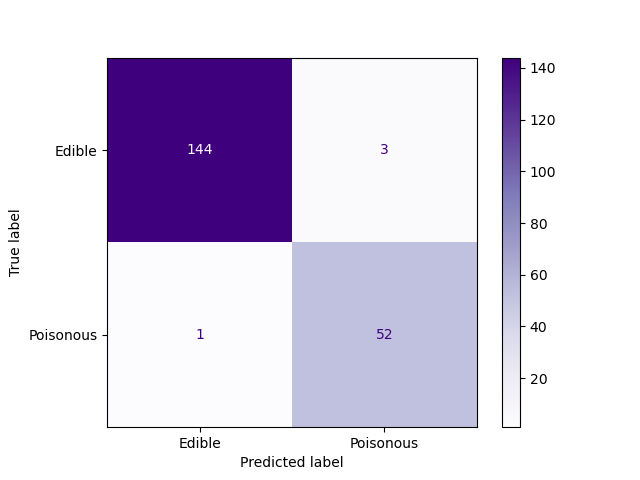
\includegraphics[width=0.6\linewidth]{Images/ImprovedNet_ConfusionMatrix.png}
    \caption{Konfúzna matica ImprovedNet ("Vylepšeného" modelu)}
    \label{fig:enter-label}
\end{figure}

Z výsledkov je vidno, že naša modifikácia nebola až taká prínosná ako sme si mysleli. Výsledky neindikujú žiadnu substačnú zmenu vo výkone modelu. V našom prípade boli dokonca všetky metriky horšie oproti pôvodnému modelu, s najväčšou zmenou v čase trénovania, čo dáva zmysel pretože funkcia Swish je viac počítačovo námahová oproti ReLU. Tento výsledok nám však dáva informáciu že miznujúce gradienty niesu veľkým problémom pre náš model.

\section{Záver}
\IEEEPARstart{P}{ropozovaný} model popísaný v článku sme implemetovali, trénovali a testovali na poskytnutom dataset-e. Jeho výsledky sme porovnali s 3 predtrénovanímy architektúrami AlexNet, ResNet50, a GoogleNet (InceptionV1) ktoré boli všetky pretrénované na dataset pomocou transfer learning. Súčasťou výsledkov tiež bola aj priemerná trénovacia presnosť získaná pomocou k-fold cross validation datasetu a tiež aj efektívnosť modelov ako súčasť procesu RCNN. Napriek viacero implemetačných rozdielov ktoré vznikli ako dôsledok nedostatku informácií z pôvodného článku, sme získali výsledky ktoré boli podobné pôvodnému článku a tým pádom sme aj došli k rovnakému záveru. Propozovaný model síce nevedel dosiahnuť väčšiu presnosť ako predtrénované architektúry ale vedel získať podobné hodnoty presnosti za najmenší čas, 99.00 \% za 40s pre CNN, a 95.00 \%  za 2min 39s pre RCNN.

\vspace{10pt}

\IEEEPARstart{}{} Nakoniec sme sa pokusili vylepšiť pôvodný model pomocou zmeny aktivačnej funkcie, čo nemalo žiadny vplyv na výkon modelu ale uistili sme sa tým že v modeli nedochádza k problému miznujúcich gradientov.

\vspace{10pt}

\IEEEPARstart{}{} Touto replikáciou sme došli k tomu že architektúra propozovaného modelu je vhodná a replikovatelná, odporúčame ju na použitie v klasifikačných problémoch hlavne kde záleží na čase trénovania modelu. 

\ifCLASSOPTIONcaptionsoff
  \newpage
\fi

\begin{thebibliography}{4}

\bibitem{pc}
A New Deep Learning Model for the Classification of
Poisonous and Edible Mushrooms Based on Improved AlexNet
Convolutional Neural Network [\url{https://www.mdpi.com/2076-3417/12/7/3409}]

\bibitem{wk}
Wacharaphol Ketwongsa [\url{https://orcid.org/0000-0002-5254-9869}]

\bibitem{uk}
Urachart Kokaew [\url{https://orcid.org/0000-0003-3900-6453}]

\bibitem{kk}
Khon kaen univerzita [\url{https://www.kku.ac.th/}]

\bibitem{nc}
Nový čas, Toxíny v sebe nemajú iba muchotrávky: Lekárka radí, čo robiť, ak sa otrávite hubami [\url{https://www.cas.sk/clanok/2842865/toxiny-v-sebe-nemaju-iba-muchotravky-lekarka-radi-co-robit-ak-sa-otravite-hubami?orig_gallery_article=1}]

\bibitem{mz}
Nahuby.sk, Igor Hlavatý [\url{https://www.nahuby.sk/obrazok_detail.php?obrazok_id=720143&poradie=7&form_hash=15ae8dde5a27dfbc1b3e25a7f8234e08}]

\bibitem{mc}
Nahuby,sk, Mirosloav Valent [\url{https://www.nahuby.sk/obrazok_detail.php?obrazok_id=805855&poradie=5&form_hash=bd6e91af4351fd68128857cc0969fbaf}]

\bibitem{swish}
Graf aktivačnej funkcie Swish a jej derivácie [\url{https://www.superannotate.com/blog/activation-functions-in-neural-networks}]

\end{thebibliography}
\end{document}